\begin{surferPage}[30 Cuspides]{A S\^extica de  Barth com 30 C\'uspides}
    Depois de Wolf Barth ter constru\'ido a s\^extica com o n\'umero m\'aximo poss\'ivel de singularidades, $65$ (ver essa superf\'icie nesta galeria) e depois
    de dois dos seus alunos de doutoramento tamb\'em terem constru\'ido novas superf\'icies recordistas mundiais para graus mais elevados, Barth come\c cou a colocar a quest\~ao acerca do n\'umero m\'aximo de c\'uspides de superf\'icies de um determinado grau.

   A constru\c c\~ao da s\^extica de Barth com $65$ singularidades do tipo
    $A_1^{+-}$ (cones duplos) pode ser adaptada para c\'uspides, resultando em $30$ c\'uspides: 
    \[P_6 - \alpha \cdot K^3=0,\]
  onde $P_6$ s\~ao os mesmos planos de simetria do icosaedro, como para a  outra S\^extica de Barth, e onde $K$ \'e novamente a equa\c c\~ao da esfera unit\'aria:
    \vspace*{-0.4em}
    \begin{center}
      \begin{tabular}{c@{\ }c@{\ }c@{\ }c}
        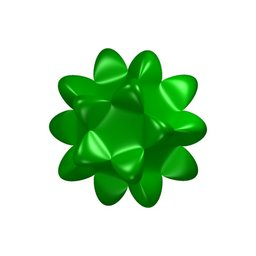
\includegraphics[height=1.2cm]{./../../common/images/barthsextic_30A2}
        &
        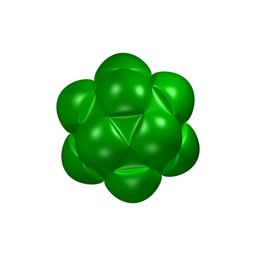
\includegraphics[height=1.2cm]{./../../common/images/barthsextic_30A2_3}
        &
        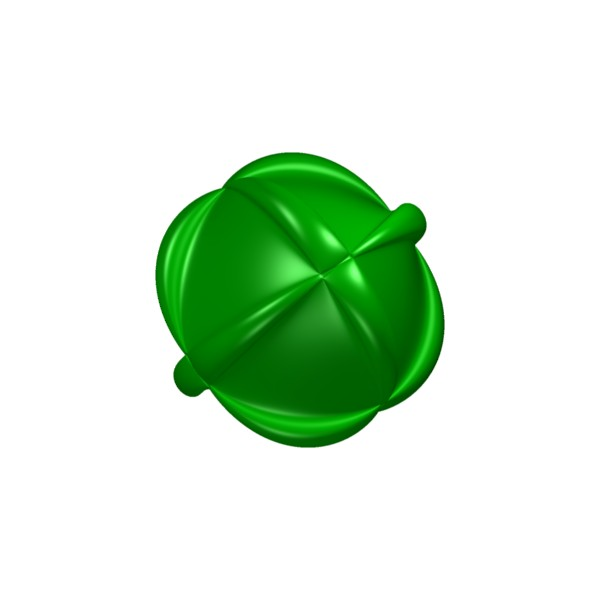
\includegraphics[height=1.2cm]{./../../common/images/barthsextic_30A2_5}
        &
        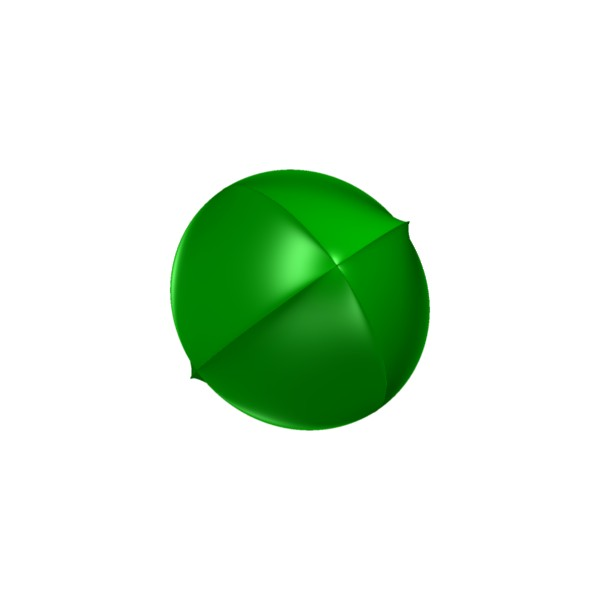
\includegraphics[height=1.2cm]{./../../common/images/barthsextic_30A2_6}
      \end{tabular}
    \end{center}    
    \vspace*{-0.3em}
     Este \'e o atual recorde mundial para o n\'umero m\'aximo de c\'uspides reais em s\^exticas. Para c\'uspides complexas,  o recorde mundial \'e de $36$.
\end{surferPage}
